\documentclass[10pt]{article}

\usepackage[letterpaper,margin=0.62in]{geometry}
\usepackage[T1]{fontenc}
\usepackage{lmodern}
\usepackage{microtype}
\usepackage[table]{xcolor}
\usepackage{enumitem}
\usepackage{tabularx}
\usepackage{array}
\usepackage{booktabs}
\usepackage{tikz}
\usepackage[hidelinks]{hyperref}
\usetikzlibrary{arrows.meta,positioning,fit,calc}

\definecolor{navy}{HTML}{17365D}
\definecolor{blue}{HTML}{2F75B5}
\definecolor{lightblue}{HTML}{D9EAF7}
\definecolor{paleblue}{HTML}{EFF6FB}
\definecolor{lightgray}{HTML}{F2F4F7}
\definecolor{textgray}{HTML}{374151}

\setlength{\parindent}{0pt}
\setlength{\parskip}{3pt}
\setlist[itemize]{leftmargin=1.25em,itemsep=1pt,topsep=2pt}
\renewcommand{\arraystretch}{1.13}
\pagestyle{plain}

\newcommand{\sectiontitle}[1]{%
  \vspace{3pt}{\large\bfseries #1}\par\vspace{1pt}}

\begin{document}

{\LARGE\bfseries Planning Report for a Generic Auction Simulator}\par
{\large\bfseries\color{navy} Programmed and LLM Based Agents}\par\vspace{5pt}

\begin{tabularx}{\textwidth}{>{\bfseries\color{navy}}p{0.75in} X >{\bfseries\color{navy}}p{0.85in} X}
\rowcolor{lightblue}
Code & HAN2601 & Supervisor & Prof. ZHANG Hanrui \\
Students & LIU Xianlong and MA Ho Tsun Matthew & Submission & 30 September 2026 \\
\end{tabularx}

\sectiontitle{Project Goal}
The project will develop a web-based auction simulator in which an auctioneer and multiple bidders communicate through a common message protocol. The complete platform is intended to support both programmed agents and large language model agents. The first version will deliberately use only a fixed scripted auctioneer and scripted bidders. This narrower scope will allow the team to verify message delivery, synchronous turn handling, auction rules, allocation, payment and profit calculation before adding the uncertainty and cost of LLM calls.

\sectiontitle{Significance of the Project}
\textbf{What.} The project provides a reusable environment for running and observing auctions under controlled rules and valuations. \textbf{Who.} Students and researchers can use it to compare bidding strategies, inspect complete auction histories and later evaluate LLM agents under the same conditions as programmed baselines. \textbf{Why.} Existing experiments often combine communication, auction logic and strategy in one implementation, which makes failures difficult to isolate and results difficult to reproduce. A common receiver and message format will separate these concerns and create a reliable baseline for later intelligent agents.

\sectiontitle{Problem Statement}
An auction involves messages from both the auctioneer and bidders, but those messages must be processed in the correct session, round and order. Without central coordination, two bidders may act at the same time, an out-of-date bid may be accepted, or one agent may see information that should remain private. The backend must therefore receive every message, verify its sender and context, route it to the correct participant, and synchronize the next action. It must also keep the auction state and event history consistent if an agent sends an invalid message or fails to respond.

\sectiontitle{Proposed Solution and Deliverables}
\begin{itemize}
  \item \textbf{Receiver and synchronizer.} A central backend component will accept messages from the auctioneer and bidders, validate their envelopes, control the current turn or round, route permitted information and handle response deadlines.
  \item \textbf{Common message protocol.} Messages will contain a session identifier, sender, recipient or audience, message type, round number and structured payload. The same protocol can later carry LLM-generated actions.
  \item \textbf{Deterministic auction service.} Coded rules will maintain session state, decide whether an action is legal, calculate winners and payments, and remain the source of truth for each result.
  \item \textbf{Scripted baseline agents.} The first bidder will bid $0.8v$, where $v$ is its assigned valuation or reference price. Winning below $v$ produces a positive surplus. The next strategy stage will make the multiplier configurable in $[0.8,1.2]$ to study conservative and over-bidding behaviour.
  \item \textbf{Event log and demonstration.} Every accepted and rejected message will be recorded for replay, debugging and performance measurement. A simple interface will show the current state, messages, bids and final result.
  \item \textbf{Future LLM adapter.} After the scripted version is stable, an adapter will convert receiver observations into prompts and convert structured model output back into the same action messages. LLM work is not part of the first-version acceptance criteria.
\end{itemize}

\textbf{First-version success criteria.} A complete scripted auction can run without manual intervention; messages are processed in a valid synchronous order; invalid or late actions cannot corrupt the session; the winner, payment and profit are correct; and the event log can reproduce the observed result.

\newpage

\sectiontitle{Backend Architecture}

\begin{center}
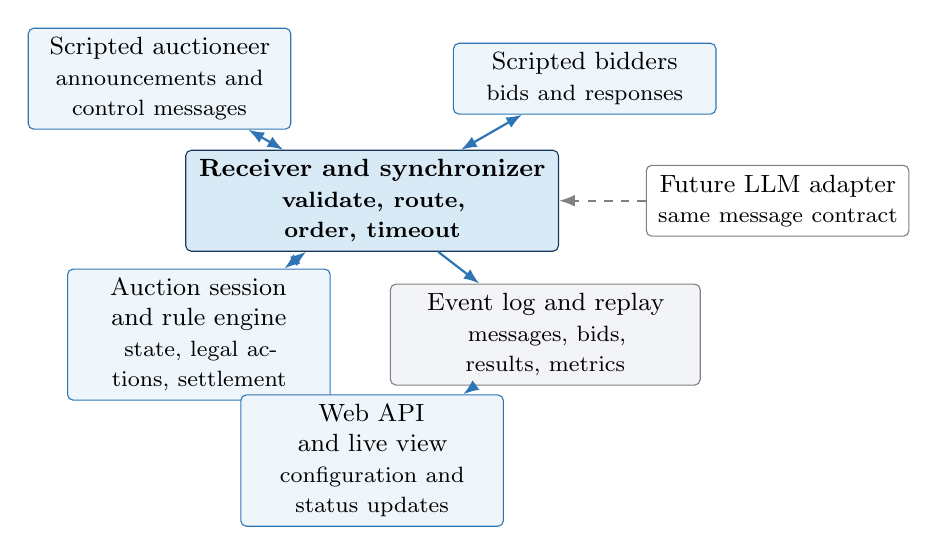
\begin{tikzpicture}[
  node distance=6mm and 8mm,
  box/.style={draw=blue, rounded corners=2pt, fill=paleblue, align=center,
              minimum height=9mm, text width=31mm, font=\small},
  core/.style={draw=navy, rounded corners=2pt, fill=lightblue, align=center,
               minimum height=12mm, text width=45mm, font=\small\bfseries},
  store/.style={draw=gray, rounded corners=2pt, fill=lightgray, align=center,
                minimum height=9mm, text width=37mm, font=\small},
  flow/.style={-{Latex[length=2mm]}, thick, draw=blue},
  biflow/.style={{Latex[length=2mm]}-{Latex[length=2mm]}, thick, draw=blue}
]
  \node[box] (auctioneer) at (-2.7,0) {Scripted auctioneer\\\footnotesize announcements and control messages};
  \node[box] (bidders) at (2.7,0) {Scripted bidders\\\footnotesize bids and responses};
  \node[core] (receiver) at (0,-1.55) {Receiver and synchronizer\\\footnotesize validate, route, order, timeout};
  \node[box] (rules) at (-2.2,-3.25) {Auction session and rule engine\\\footnotesize state, legal actions, settlement};
  \node[store] (events) at (2.2,-3.25) {Event log and replay\\\footnotesize messages, bids, results, metrics};
  \node[box] (api) at (0,-4.85) {Web API and live view\\\footnotesize configuration and status updates};
  \node[box, draw=gray, fill=white] (future) at (5.15,-1.55) {Future LLM adapter\\\footnotesize same message contract};

  \draw[biflow] (auctioneer) -- (receiver);
  \draw[biflow] (bidders) -- (receiver);
  \draw[biflow] (receiver) -- (rules);
  \draw[flow] (receiver) -- (events);
  \draw[flow] (events) -- (api);
  \draw[flow, dashed, draw=gray] (future) -- (receiver);
\end{tikzpicture}
\end{center}

The receiver is the communication boundary for the whole simulation. An agent never changes the auction state directly. It sends an action message to the receiver, which checks the session and round, asks the deterministic rule engine to validate and apply the action, records the outcome, and then releases the next permitted message. This design provides synchronous behaviour even if the internal components later use asynchronous network calls.

\textbf{Suggested implementation.} The first release can be a modular Python backend with a REST API and a WebSocket event stream. The receiver, auction rules, scripted strategies and event store should be separate modules inside one deployable application. SQLite is sufficient for the prototype; a larger database or worker queue should be added only if experiment volume requires it.

\sectiontitle{Proposed Timeline}
\begin{tabularx}{\textwidth}{>{\raggedright\arraybackslash}p{1.35in} >{\raggedright\arraybackslash}p{1.65in} X}
\rowcolor{navy}
\color{white}\bfseries Period & \color{white}\bfseries Work package & \color{white}\bfseries Expected output \\
24 Sep--11 Oct 2026 & Protocol and architecture & Message schema, receiver interfaces, session states and automated test plan \\
\rowcolor{lightgray}
12 Oct--8 Nov 2026 & Scripted vertical slice & Fixed auctioneer, $0.8v$ bidder, synchronous receiver and one complete auction \\
9 Nov--6 Dec 2026 & Auction rules & Required sealed-bid mechanisms, validation, settlement and invariant tests \\
\rowcolor{lightgray}
7 Dec 2026--17 Jan 2027 & Strategy experiments & Configurable multiplier in $[0.8,1.2]$, repeatable scenarios and profit metrics \\
18 Jan--21 Feb 2027 & Dynamic auctions and storage & English, Dutch and Japanese flows, event log, replay and export \\
\rowcolor{lightgray}
22 Feb--31 Mar 2027 & Demonstration and testing & REST/WebSocket API, live view, failure tests and documentation \\
1 Apr 2027--final deadline & Evaluation and submission & Comparative experiments, analysis, demonstration and final report; optional LLM adapter if the baseline is stable \\
\end{tabularx}

\vspace{4pt}
\textbf{Reference.} J. Chen et al., ``Put Your Money Where Your Mouth Is: Evaluating Strategic Planning and Execution of LLM Agents in an Auction Arena,'' arXiv:2310.05746, 2024. Project page: \url{https://auction-arena.github.io/}.

\end{document}
